reinfreinf\section{Objetives}
In the second part of the mechanical characterization of composites laboratory
session, a flexural testing is performed, also called three point bending, over
4 different samples. The objective, as in the last session, is to characterize
the mechanical performance of the laminated and sandwich-like polymer matrix
composites, comparing the obtained experimental results with the calculated
theoretical ones.

\section{Development of the lab session and material used}
As in previous sessions, various samples were tested for the same material. In this session, the following samples were tested:
\begin{itemize}
	\item 3 samples of unreinforced polypropylene (1A, 1B, 1C)
	\item 3 samples of glass fiber + polypropylene (2A, 2B, 2C)
	\item 3 samples of twintex (3A, 3B, 3C)
	\item 1 sample of foam sandwich panel  (4)
	\item 1 sample of cardboard sandwich panel with honeycomb structure (5)
\end{itemize}

All of them were at the same temperature (ambient, 20ºC aprox)
and were tested at the same velocity: 5 mm/min. Their characteristics and maximum
force obtained are shown in the table \ref{tab:characteristics}.

\begin{figure}[h]
	\centering
	\begin{subfigure}{0.45\textwidth}
		\centering
		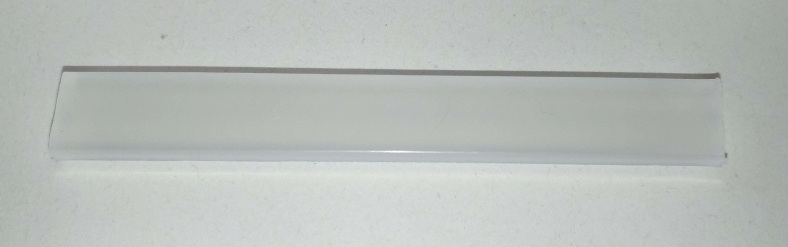
\includegraphics[width=\textwidth]{img/neat_PP.jpg}
		\caption{Unreinforced Polypropylene}
		\label{fig:uPP}
	\end{subfigure}
	~ %add desired spacing between images, e. g. ~, \quad, \qquad, \hfill etc.
	%(or a blank line to force the subfigure onto a new line)
	\begin{subfigure}{0.45\textwidth}
		\centering
		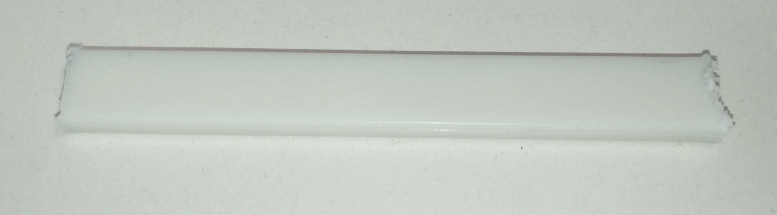
\includegraphics[width=\textwidth]{img/reinf_PP.jpg}
		\caption{Reinforced Polypropylene}
		\label{fig:rPP}
	\end{subfigure}
	\\
	\begin{subfigure}{0.6\textwidth}
		\centering
		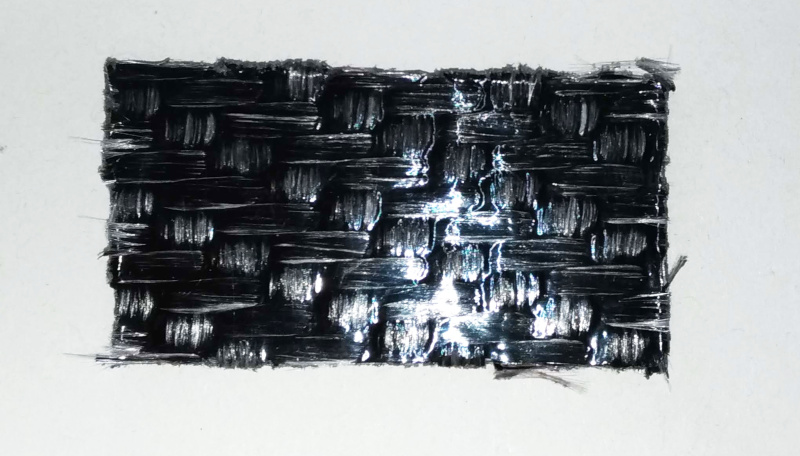
\includegraphics[width=\textwidth]{img/Twintex.jpg}
		\caption[short caption]{Twintex}
		\label{fig:twintex}
	\end{subfigure}
	\\
	\begin{subfigure}{0.45\textwidth}
		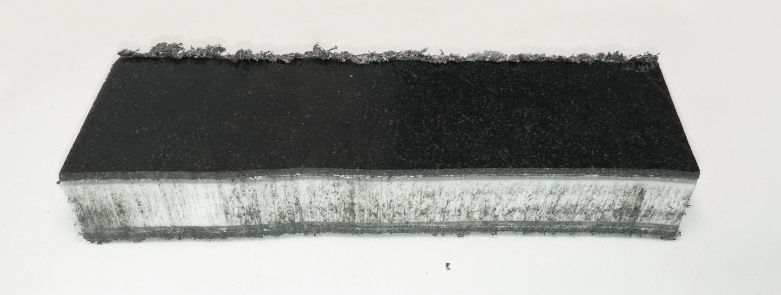
\includegraphics[width=\textwidth]{img/foam_sandwich.jpg}
		\caption[short caption]{Foam sandwich panel}
		\label{fig:foam_sandwich}
	\end{subfigure}
	~
	\begin{subfigure}{0.45\textwidth}
		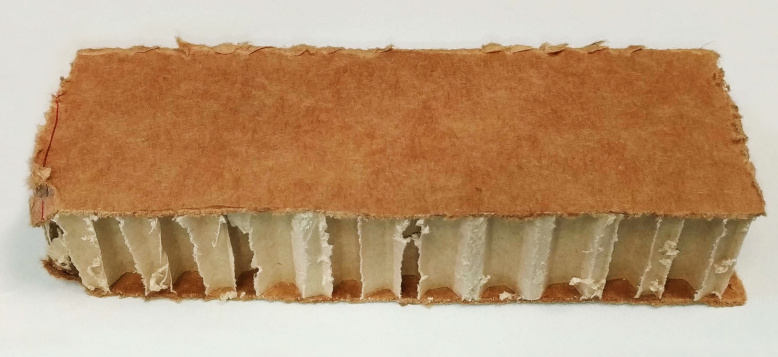
\includegraphics[width=\textwidth]{img/cardboard.jpg}
		\caption[short caption]{Cardboard panel}
		\label{fig:cardboard_sandwich}
	\end{subfigure}

	\caption{Samples before the test}
	\label{fig:cmos_transistors}
\end{figure}

\begin{table}[]
\centering
\begin{tabular}{ccccc}
\hline
\textbf{Sample} & \textbf{Width(mm)} & \textbf{Thickness(mm)} & \textbf{Span(mm)} & \textbf{Max load (N)} \\ \hline
\textbf{1A}     & 10.5               & 4.3                    & 68.8              & 83.3                   \\ \hline
\textbf{1B}     & 10.5               & 4.4                    & 70.4              & 84.5                   \\ \hline
\textbf{1C}     & 10.5               & 4.4                    & 70.4              & 85.0                   \\ \hline
\textbf{2A}     & 10.5               & 4.4                    & 70.4              & 267.0                  \\ \hline
\textbf{2B}     & 10.5               & 4.4                    & 70.4              & 269.0                  \\ \hline
\textbf{2C}     & 10.5               & 4.4                    & 70.4              & 266.0                  \\ \hline
\textbf{3A}     & 27.2               & 2.3                    & 36.8              & 330.0                  \\ \hline
\textbf{3B}     & 28.3               & 2.4                    & 38.4              & 250.0                  \\ \hline
\textbf{3C}     & 28.1               & 2.5                    & 40.0              & 300.0                  \\ \hline
\textbf{4}      & 40.0               & 19.6                   & 80                & 3995                   \\ \hline
\textbf{5}      & 57.0               & 30.7                   & 114.0             & 348			\\ \hline
\end{tabular}
\caption{Characteristics and maximum force tested during the laboratory session}
\label{tab:characteristics}
\end{table}

During this session a three point bending test was performed, using the universal
testing machine (UTM) and following ISO 178 and ASTM C393 (Figure \ref{fig:machine}:
PP reinforced sample being tested).

\begin{figure}[h]
	\centering
	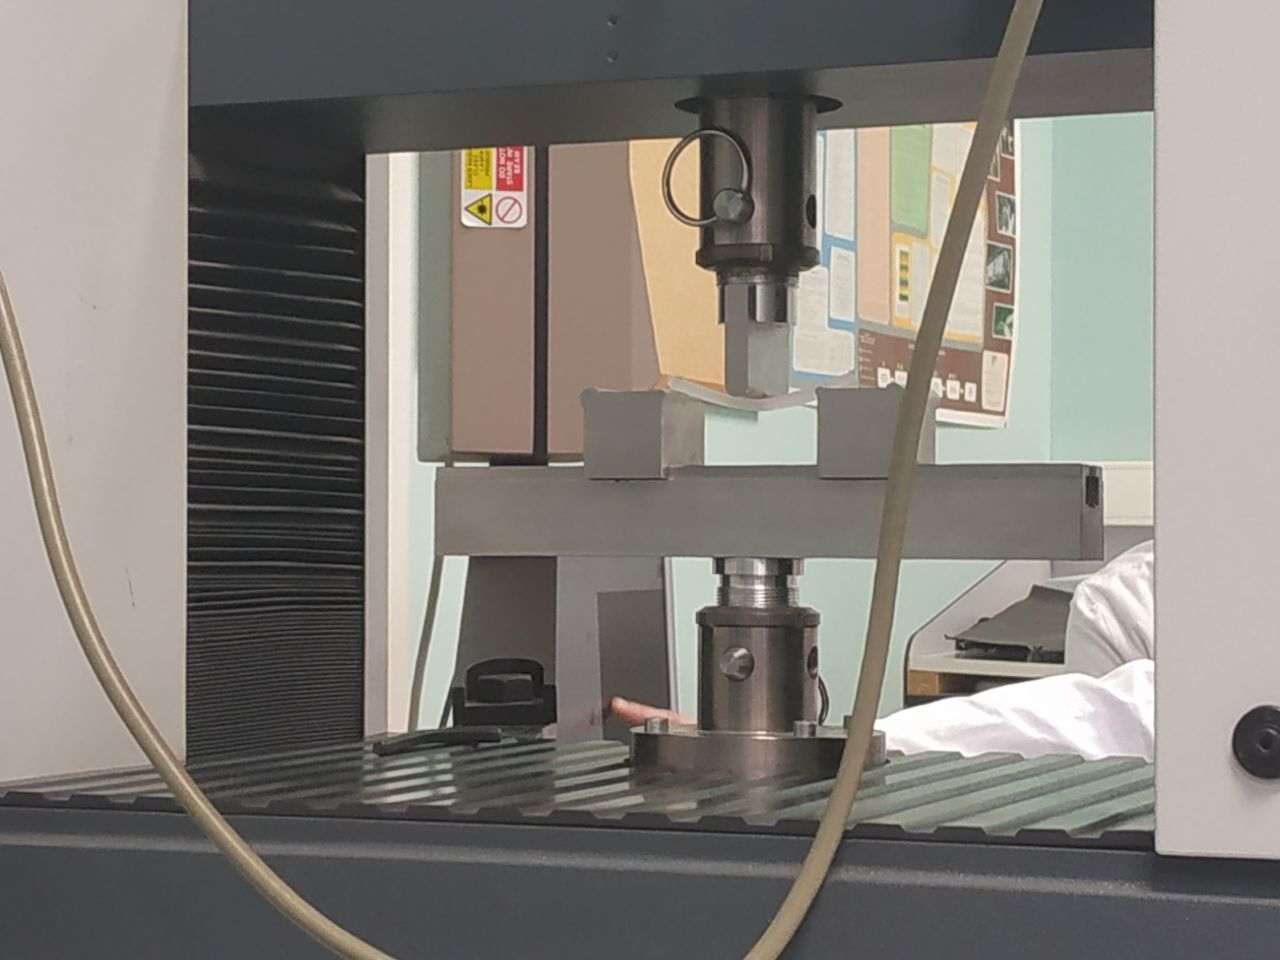
\includegraphics[width=0.6\textwidth]{img/machine.jpg}
	\caption{PP reinforced sample being tested}
	\label{fig:machine}
\end{figure}

This test consists in applying a force in the sample generating a bend (see Figure \ref{fig:3point_bending}).
The separation of the supporting pins, called span, is 2 times the width for the
sandwich samples, and 16 times the thickness for the other samples.


\begin{figure}[h]
	\centering
	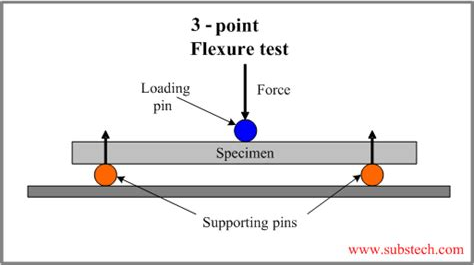
\includegraphics[width=0.6\textwidth]{img/schema.png}
	\caption{Scheme of the three point bending test}
	\label{fig:3point_bending}
\end{figure}

With this test values for the modulus of elasticity in bending, flexural stress,
flexural strain, and the flexural stress–strain response of the material are obtained.
It has to be noted that unlike the tensile testing, this test does not have
specific requirements regarding sample shape, but the position of the loads
has to be considerate in order to not disrupt the results.

\clearpage

\section{Questions}

Using the rule of mixtures, the theoretical values of the materials can be
calculated in order to compare the results with the experimental ones.

For a 2 component composite $V_m + V_f = 1$:

\begin{equation}
	E_c = E_m V_m + E_f V_f
\end{equation}

\begin{equation}
	\frac{1}{E_c} = \frac{V_m}{E_m} + \frac{V_f}{E_f}
\end{equation}

And knowing the values of the characteristics for the matrix and fiber,
the values obtained can be found in the table \ref{tab:theoretical}.

\begin{table}[h]
\begin{tabular}{cccc}
\hline
\textbf{Sample}                 & \textbf{Vf} & \textbf{Young Modulus (GPa)} & \textbf{Shear Core Stress ($N/mm^2$)} \\ \hline
\textbf{Polypropylene (PP)}     & -             & 1.5                          & -                            	\\ \hline
\textbf{Glass Fiber (GF)}       & -             & 69                           & -                            	\\ \hline
\textbf{PP+30\% GF}            & 0.3           & 21.75                        & -                             	\\ \hline
\textbf{Twintex}                & 0.6           & 42                           & -                            	\\ \hline
\textbf{Polypropylene Sandwich} & -             & -                            & 5.0957                       	\\ \hline
\textbf{Cardboard Sandwich}     & -             & -                            & 0.1989				\\ \hline
\end{tabular}
\caption{Theoretical values obtained with the rule of mixture}
\label{tab:theoretical}
\end{table}

\begin{figure}[h]
	\centering
	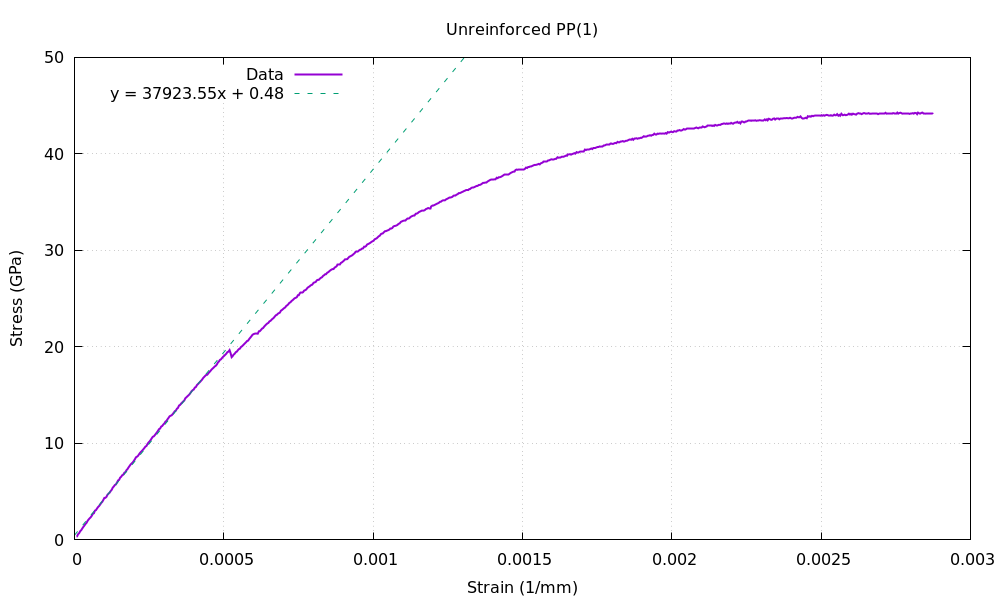
\includegraphics[width=0.8\textwidth]{img/neat_PP1.png}
	\caption{Experimental data for Unreinforced polypropylene 1}
\end{figure}
\begin{figure}[h]
	\centering
	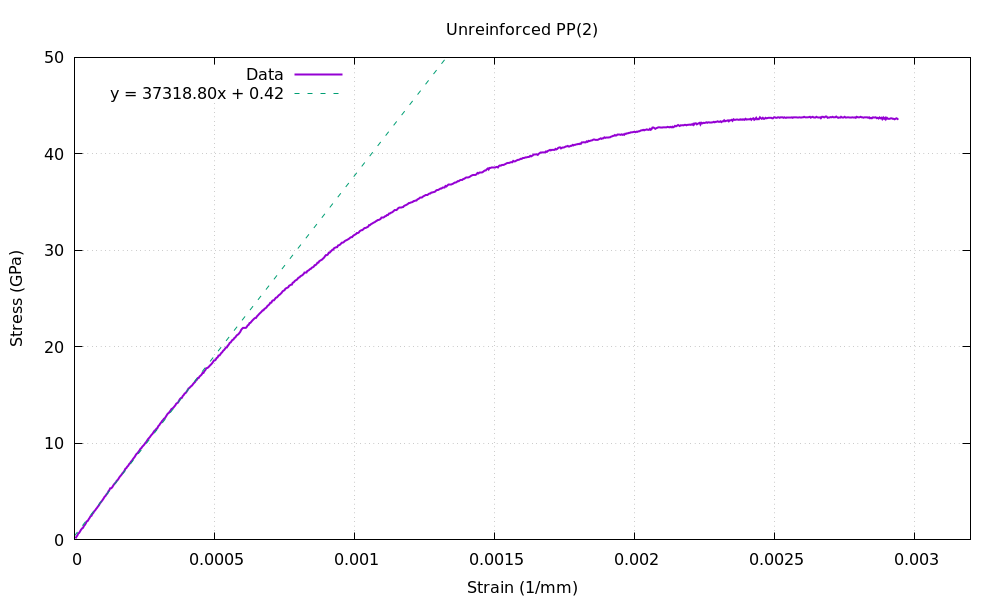
\includegraphics[width=0.8\textwidth]{img/neat_PP2.png}
	\caption{Experimental data for Unreinforced polypropylene 2}
\end{figure}
\begin{figure}[h]
	\centering
	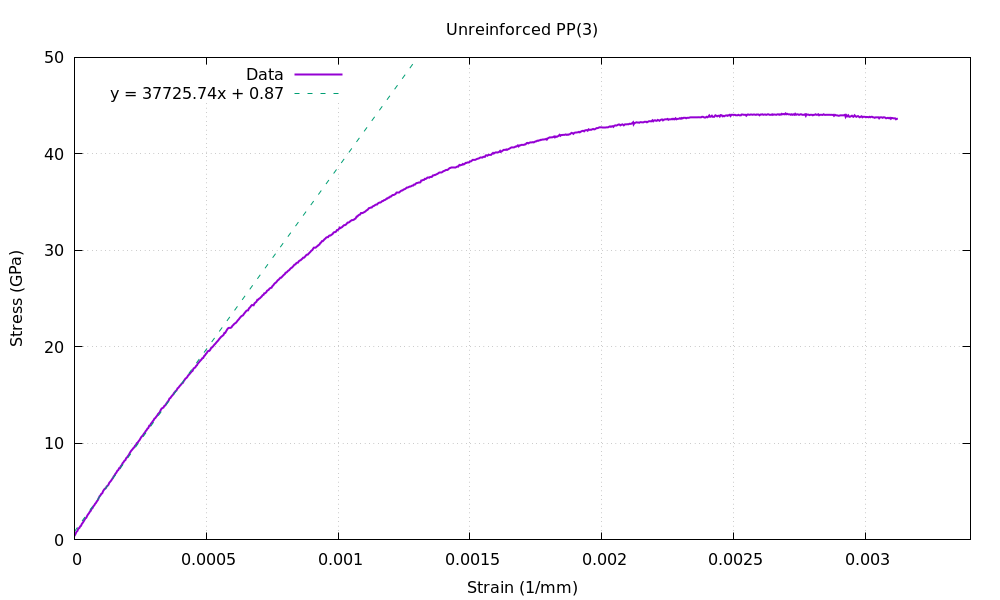
\includegraphics[width=0.8\textwidth]{img/neat_PP3.png}
	\caption{Experimental data for Unreinforced polypropylene 3}
\end{figure}
\begin{figure}[h]
	\centering
	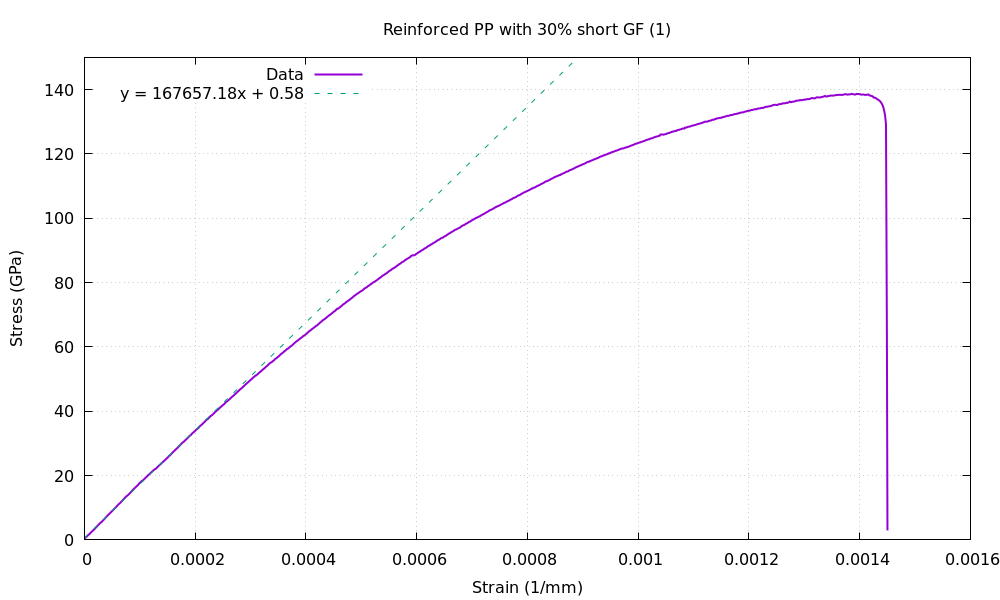
\includegraphics[width=0.8\textwidth]{img/reinf_PP1.png}
	\caption{Experimental data for reinforced polypropylene 1}
\end{figure}
\begin{figure}[h]
	\centering
	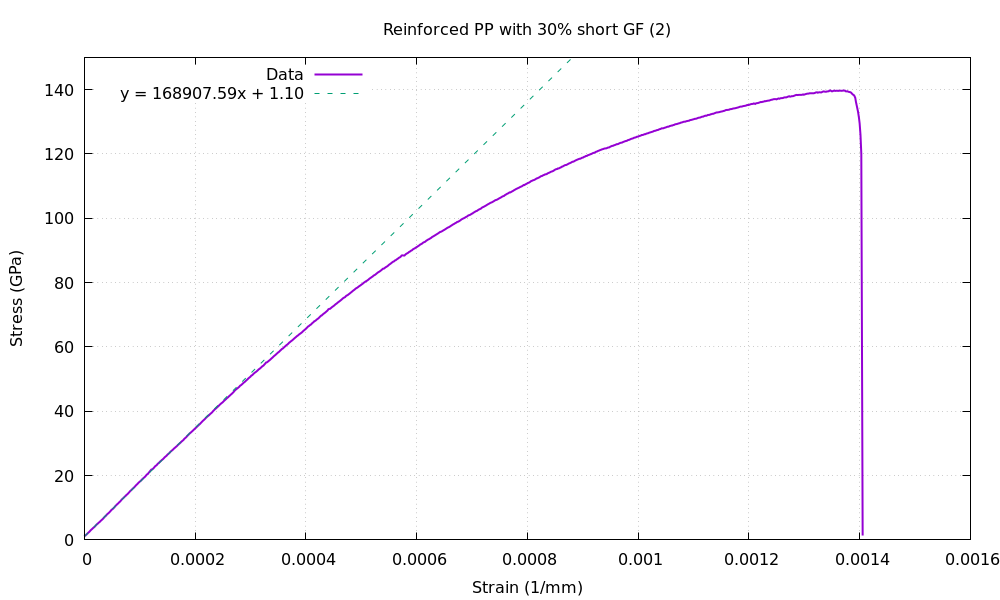
\includegraphics[width=0.8\textwidth]{img/reinf_PP2.png}
	\caption{Experimental data for reinforced polypropylene 2}
\end{figure}
\begin{figure}[h]
	\centering
	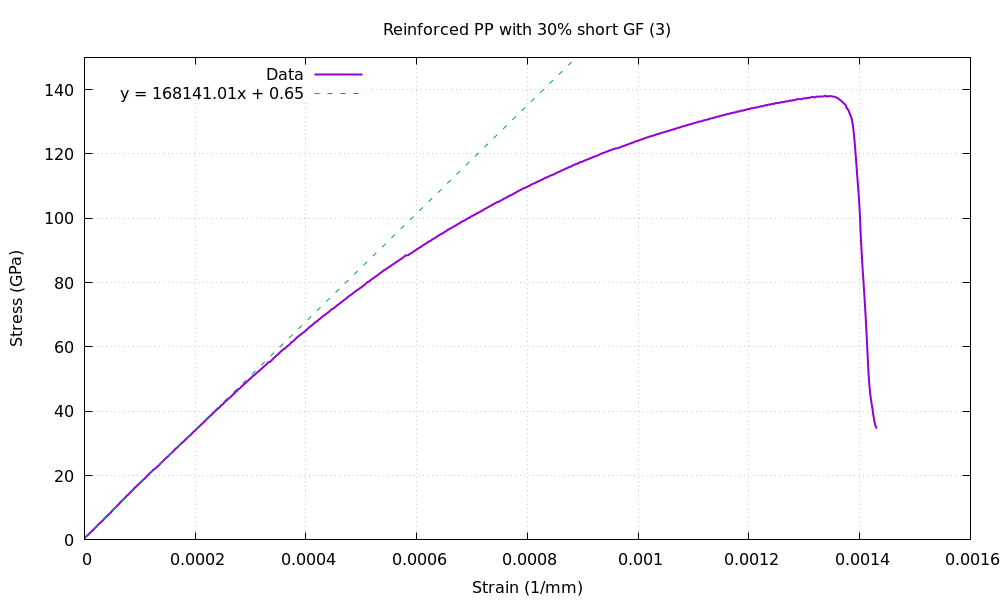
\includegraphics[width=0.8\textwidth]{img/reinf_PP3.png}
	\caption{Experimental data for reinforced polypropylene 3}
\end{figure}

\begin{figure}[h]
	\centering
	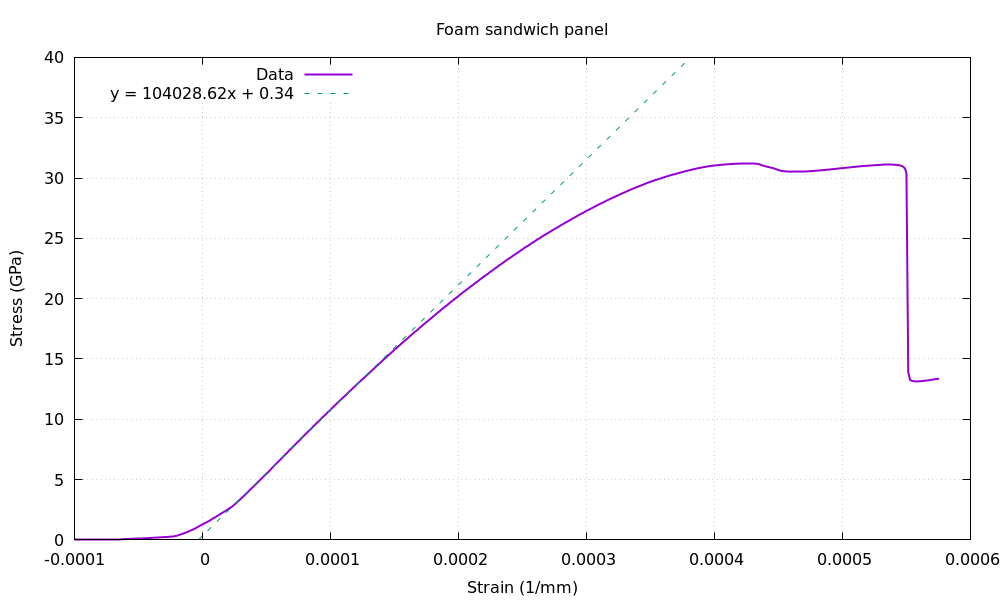
\includegraphics[width=0.8\textwidth]{img/foam_sandwich.png}
	\caption{Experimental data for foam core sandwich}
\end{figure}

\begin{figure}[h]
	\centering
	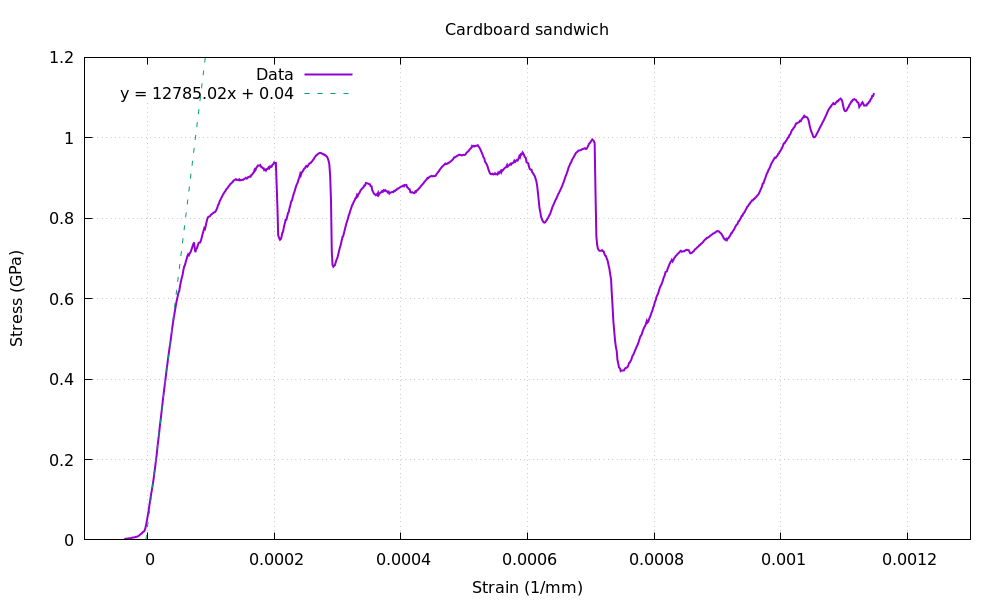
\includegraphics[width=0.8\textwidth]{img/cardboard_sandwich.png}
	\caption{Experimental data for cardboard sandwich}
\end{figure}


\clearpage
\section{Conclusions}

Even though the range of values for the young modulus for the polypropylene and glass fiber cover a wide range of values, there is an average around them
that is to be close to what we have measured and so we can call the lab practice a success. The strain-stress curves are as expected, where we can also see
the microcraking starting on the little peaks.

For the sandwiches, there could be seen that, as we expected, the polypropylene sandwich has a greater shear core stress than the cardboard sandwich,
this may be because of the materials that they were made of. To be noticed is that the shear core stress of the cardboard sandwich was bigger than one
could expect from its materials.
